% Use the following line _only_ if you're still using LaTeX 2.09.
%\documentstyle[icml2017,epsf,natbib]{article}
% If you rely on Latex2e packages, like most moden people use this:
\documentclass{article}

% use Times
\usepackage{times}
% For figures
\usepackage{graphicx} % more modern
%\usepackage{epsfig} % less modern
\usepackage{subfigure}

% For citations
\usepackage{natbib}

% For algorithms
\usepackage{algorithm}
\usepackage{algorithmic}

% As of 2011, we use the hyperref package to produce hyperlinks in the
% resulting PDF.  If this breaks your system, please commend out the
% following usepackage line and replace \usepackage{icml2017} with
% \usepackage[nohyperref]{icml2017} above.
\usepackage{hyperref}

% Packages hyperref and algorithmic misbehave sometimes.  We can fix
% this with the following command.
\newcommand{\theHalgorithm}{\arabic{algorithm}}

% Employ the following version of the ``usepackage'' statement for
% submitting the draft version of the paper for review.  This will set
% the note in the first column to ``Under review.  Do not distribute.''
\usepackage{icml2017}

% Employ this version of the ``usepackage'' statement after the paper has
% been accepted, when creating the final version.  This will set the
% note in the first column to ``Proceedings of the...''
%\usepackage[accepted]{icml2017}


%%%%%%%%%%%%%%%%%%%%%%%%%%%%%%%%%
% Custom packages
%%%%%%%%%%%%%%%%%%%%%%%%%%%%%%%%%
% AKM: already present above!
%\usepackage{hyperref}
\usepackage{amsmath}
\usepackage{amsfonts}
\usepackage{mathrsfs}
\usepackage{bm}
\usepackage{bbm}
\usepackage{stmaryrd}
\usepackage{algorithm}
\usepackage{algorithmic}
%\usepackage[sc]{mathpazo}
%\linespread{1.05}         % Palladio needs more leading (space between lines)
\usepackage[T1]{fontenc}    % use 8-bit T1 fonts
%\usepackage{subcaption}  % sub-figures
\usepackage{nicefrac}       % compact symbols for 1/2, etc.
\usepackage{microtype}      % microtypography
\usepackage{booktabs} % professional-quality tables
\graphicspath{{fig/}} % Location of the graphics files

\usepackage{enumitem}

%%%%%%%%%%%%%%%%%%%%%%%%%%%%%%%%%
% Custom notation
%%%%%%%%%%%%%%%%%%%%%%%%%%%%%%%%%
\DeclareMathOperator*{\argmin}{argmin}
\DeclareMathOperator*{\argmax}{argmax}
\newcommand{\given}{\mid}
\newcommand{\llb}{\llbracket}
\newcommand{\rrb}{\rrbracket}
\newcommand{\indicator}[1]{\llbracket #1 \rrbracket}
\newcommand{\eat}[1]{}
\newcommand{\Q}{\mathsf{Q}}
\newcommand{\X}{\mathsf{X}}
\newcommand{\Y}{\mathsf{Y}}
\newcommand{\CCal}{\mathscr{C}}
\newcommand{\QCal}{\mathscr{Q}}
\newcommand{\XCal}{\mathscr{X}}
\newcommand{\YCal}{\mathscr{Y}}
\newcommand{\SSf}{\mathsf{S}}
\newcommand{\Real}{\mathbb{R}}
\newcommand{\E}[2]{\underset{#1}{\mathbb{E}}\left[ #2 \right]}
\newcommand{\ES}[2]{\underset{#1}{\mathbb{E}}\, #2}

% madeness: suPer-script in Brackets
\newcommand{\pb}[1]{^{({#1})}}

\newcommand{\bu}{\mathbf{u}}
\newcommand{\bv}{\mathbf{v}}
\newcommand{\x}{\mathbf{x}}
\newcommand{\y}{\mathbf{y}}
\newcommand{\w}{\mathbf{w}}

\newcommand{\eg}{e.g.\ }
\newcommand{\ie}{i.e.\ }

\newcommand{\TODO}[1]{ {\color{blue}{\bf TODO:~{#1}}} }



% The \icmltitle you define below is probably too long as a header.
% Therefore, a short form for the running title is supplied here:
\icmltitlerunning{Sequence Recommendation with Structured Prediction}

\begin{document}

\twocolumn[
\icmltitle{Sequence Recommendation with Structured Prediction}
%\icmltitle{Structured Recommendation}

% It is OKAY to include author information, even for blind
% submissions: the style file will automatically remove it for you
% unless you've provided the [accepted] option to the icml2017
% package.

% list of affiliations. the first argument should be a (short)
% identifier you will use later to specify author affiliations
% Academic affiliations should list Department, University, City, Region, Country
% Industry affiliations should list Company, City, Region, Country

% you can specify symbols, otherwise they are numbered in order
% ideally, you should not use this facility. affiliations will be numbered
% in order of appearance and this is the preferred way.
\icmlsetsymbol{equal}{*}

\begin{icmlauthorlist}
\icmlauthor{Aeiau Zzzz}{equal,to}
\icmlauthor{Bauiu C.~Yyyy}{equal,to,goo}
\icmlauthor{Cieua Vvvvv}{goo}
\icmlauthor{Iaesut Saoeu}{ed}
\icmlauthor{Fiuea Rrrr}{to}
\icmlauthor{Tateu H.~Yasehe}{ed,to,goo}
\icmlauthor{Aaoeu Iasoh}{goo}
\icmlauthor{Buiui Eueu}{ed}
\icmlauthor{Aeuia Zzzz}{ed}
\icmlauthor{Bieea C.~Yyyy}{to,goo}
\icmlauthor{Teoau Xxxx}{ed}
\icmlauthor{Eee Pppp}{ed}
\end{icmlauthorlist}

\icmlaffiliation{to}{University of Torontoland, Torontoland, Canada}
\icmlaffiliation{goo}{Googol ShallowMind, New London, Michigan, USA}
\icmlaffiliation{ed}{University of Edenborrow, Edenborrow, United Kingdom}

\icmlcorrespondingauthor{Cieua Vvvvv}{c.vvvvv@googol.com}
\icmlcorrespondingauthor{Eee Pppp}{ep@eden.co.uk}

% You may provide any keywords that you
% find helpful for describing your paper; these are used to populate
% the "keywords" metadata in the PDF but will not be shown in the document
\icmlkeywords{structured prediction, sequence recommendation}

\vskip 0.3in
]

% this must go after the closing bracket ] following \twocolumn[ ...

% This command actually creates the footnote in the first column
% listing the affiliations and the copyright notice.
% The command takes one argument, which is text to display at the start of the footnote.
% The \icmlEqualContribution command is standard text for equal contribution.
% Remove it (just {}) if you do not need this facility.

\printAffiliationsAndNotice{}  % leave blank if no need to mention equal contribution
%\printAffiliationsAndNotice{\icmlEqualContribution} % otherwise use the standard text.
%\footnotetext{hi}

\begin{abstract}
% !TEX root = ./main.tex

Current recommender systems largely focus on static, unstructured content.
In many recommendation scenarios, we would like to predict content that has sequential structure,
such as when recommending a playlist of songs, or a trajectory of points-of-interest in a city.
We propose an approach to such sequential recommendation problems based on techniques from structured prediction.
While the problem can be cast as a classic structured support vector machine,
we propose two changes to the method originally designed for classification,
enabling us to solve structured recommendation problems.
First, we modify the training objective to account for the existence of multiple ground truths.
Second, we modify the prediction and loss augmented inference procedures to avoid predicting loops in the sequence via an extension of the classic Viterbi algorithm.
Experiments on two real-world trajectory recommendation datasets shows the benefits of our approach over existing, non-structured recommendation approaches.

\end{abstract}

%!TEX root = main.tex

\section{Introduction}
\label{sec:intro}

Content recommendation has been the subject of a rich body of literature~\citep{Goldberg:1992,Sarwar:2001,Koren:2010},
with established techniques seeing widespread adoption in large e-commerce companies~\citep{Linden:2003,Agarwal:2013,Amatriain:2015,Gomez-Uribe:2015}.
The success of these methods is explained by both the explosion in availability of user's explicit and implicit preferences for content,
as well as the design of methods that can suitably exploit these to make useful recommendations~\citep{Koren:2009}.

For the most part, models for recommendation have been been limited to the case of static, \emph{unstructured} content.
While this setting has considerable value by itself,
in many important scenarios one needs to recommend content that possesses some \emph{structure}.
In its simplest form, this structure may be manifest by the items we wish to recommend being \emph{sequential} in nature.
For example, consider the problem of recommending a playlist of songs to users based on their listening history~\citep{McFee:2011,chen2012playlist},
or alternately,
recommending a trajectory of points of interest in a city to a visitor~\citep{lu2010photo2trip,lu2012personalized,ijcai15,cikm16paper}.

A na\"{i}ve approach to such sequential recommendation problems is to simply ignore the structure,
and learn a standard recommendation model.
In the playlist example, we could learn a user's preference for individual songs,
and then create a playlist based on the top ranked songs.
However, it is easy to construct cases where such an approach is sub-optimal:
%This however completely ignores the fact that while a user's
for example, while a user's two favourite songs might belong
the metal and country genres respectively,
it is questionable that a playlist featuring these songs in succession will be as enjoyable to the user.
Similarly, in the trajectory recommendation problem, it is unlikely a user will want to visit three restaurants in a row.

The above raises the question of how one can effectively learn from such sequential content.
In this paper, we show how to cast sequence recommendation as a \emph{structured prediction} problem,
which allows us to leverage the toolkit of structured SVMs~\citep{tsochantaridis2005large}.
However, a vanilla application of such methods does not suffice,
as they do not account for the fact that each input can have multiple ground truths,
and the fact that \emph{loops} in predicted sequences are undesirable.
We show how one can overcome this by
suitably normalising the loss function for the model,
and by modifying the inference and prediction steps of the model using a variant of the Viterbi algorithm.
Specifically, our contributions are follows:
\begin{itemize}[noitemsep]
	\item We cast the problem of sequence recommendation as a structured prediction task, and show how this may be modelled using structured SVMs (\S\ref{sec:recseq}).
	\item We propose an important correction to the na\"{i}ve implementation of structured SVMs to the recommendation problem, so as to account for the existence of multiple ground truths for each input (\S\ref{ssec:sr}). Following \citet{joachims2009cutting} we propose both $n$-slack and 1-slack versions of the structured recommender. This new structured recommender can in principle be applied to any problem where loss augmented inference can be efficiently computed. We focus on sequence recommendation in this paper.
	\item We show how one can avoid recommending sequences with loops or repetitions via an extension of the classic Viterbi algorithm that returns a list of the highest scored sequences under some model; we show that this extension may be incorporated during both the training (via loss augmented inference) and prediction steps of our structured recommendation (\S\ref{ssec:subtour}).
	\item We explicate how trajectory recommendation can be seen as a sequential recommendation task (\S\ref{sec:trajrec}). We then present experiments on two real-world trajectory recommendation problems, and demonstrate our structured prediction approaches to offer consistent benefits over existing non-structured baselines (\S\ref{sec:experiment}).
\end{itemize}

%We begin with an overview of related work, before presenting our model.
%We begin with an overview of the sequence recommendation problem, before presenting our model.


%!TEX root = main.tex
%\section{Recommending sequences}
\section{The sequence recommendation problem}
\label{sec:recseq}

We begin with an overview of the sequence recommendation problem, before presenting our model.
Consider the following abstract
\emph{structured recommendation} problem:
given an input query $\x \in \mathcal{X}$ -- representing for example a user, a location, or some ``seed'' item --
we wish to recommend one or more \emph{structured outputs} $\y \in \mathcal{Y}$ according to a learned \emph{score function} $f(\x,\y)$.
To learn a suitable $f$,
we are provided as input a training set
%$(\x\pb{i}, \{ \y\pb{ij} \}_{j=1:n^i})$, $i=1:n$,
$\{ ( \x\pb{i}, \{ \y\pb{ij} \}_{j=1}^{n^i} ) \}_{i=1}^{n}$,
comprising a collection of inputs $\x\pb{i}$ with an associated \emph{set} of output structures $\{ \y\pb{ij} \}$.
As an example, this might represent a collection of users in a city, along with a set of trajectories that the user has visited.

For this work, we assume the output $\y$ is a \emph{sequence} of $l$ points, denoted $y_{1:l}$
where each $y_i$ belongs to some fixed set (e.g.\ places of interest in a city).
We call the resulting specialisation the \emph{sequence recommendation} problem,
and this shall be our primary interest in this paper.
The assumption that $\y$ is a sequence does not limit the generality of our approach,
as inferring $\y$ of other structure can be achieved using corresponding inference and loss-augmented inference algorithms~\cite{joachims2009predicting}.  %LX - this sentence can be cut or merged above

There are notable differences between the sequence recommendation problem and %what is being solved in
the standard problems considered in structured prediction and recommender systems.
%This setting generalises from structured prediction and recommendation problems in the following ways.
These differences bring unique challenges for both inference and learning.
In a typical structured prediction setting, the goal is to learn from a collection of $n$
input vector and output sequence tuples %$(\x\pb{i}, \y\pb{i})$, $i=1:n$.
$\{ (\x\pb{i}, \y\pb{i}) \}_{i = 1}^n$. Here,
for each distinct input $\x\pb{i}$ there is usually one \emph{unique} output sequence $\y\pb{i}$.
In a typical sequence recommendation problem, however, we expect that %learn from
%tuples $(\x\pb{i}, \{ y\pb{ij} \}_{j=1:n^i})$, $i=1:n$. That is to say,
for each input $\x\pb{i}$ (\eg users),
there %is %have not one, but a set of
are multiple associated outputs %$\{ y\pb{ij} \}_{j=1:n^i}$ (\eg movies).
$\{ \y\pb{ij} \}_{j=1}^{n^i}$ (\eg trajectories they have visited).
Indeed, the existence of multiple outputs is the basis on which even non-structured recommendation systems are built, as one looks to exploit signal embedded in the aggregate information.
For model learning, structured prediction approaches do not have a standard way to take into account multiple output sequences %$\{ \y\pb{ij} \}_{j=1:n^i}$
for each input %$\x\pb{i}$
yet.

On the other hand, for typical recommender systems problems, one assumes that the outputs are non-structured (\eg real-valued ratings for movies).
Thus, making a prediction involves enumerating all {\em non-structured} items $y$ in order to compute $\argmax_y f(\x,y)$.
For structured recommendation problems, computing $\argmax_\y f(\x,\y)$ is harder since it is often impossible to efficiently enumerate $\y$ (\eg all possible trajectories in a city).

In the rest of this section, we will first review the background of structured prediction problems (Sec~\ref{ssec:ssvm}), then present a model for structured recommendation (Sec~\ref{ssec:sr}), followed by algorithms for its learning (Sec~\ref{ssec:subtour}) and inference (Sec~\ref{ssec:SRinf}).

% In many practical
% problems we may observe more than one label for the same set of features, which violates
% the implicit assumptions of many learning algorithms. In this work we explicitly consider
% all observed labels of a particular example to be useful for training, that is we use
% the multiset of ground truths in training.
% In particular we focus on the structured prediction case,
% where the output of the classifier is from a large set $\mathcal{Y}$ with internal structure.
% An example of this is when $y\in\mathcal{Y}$ is a sequence of binary values.
% Given an example $x_i$ there may be multiple label sequences $y_{ij}$, where $j=1,...,J$.

\eat{
Suggested order:
\begin{enumerate}
  \item structured SVM
  \item multiset SSVM
  \item list Viterbi for multiple ground truths
\end{enumerate}

Then focus on trajectory
\begin{enumerate}
  \item Trajectory recommendation
  \item ILP for subtour elimination
  \item 2 uses of list Viterbi
  \begin{itemize}
    \item multiple ground truths
    \item subtour elimination
  \end{itemize}
\end{enumerate}
}

\subsection{Preliminaries: structured SVMs}
\label{ssec:ssvm}

%In structured prediction, the output of classifier given feature vector $\x$ is
%\begin{equation*}
%\y^* = \argmax_{\y \in \mathcal{Y}}~ f(\x, \y),
%\end{equation*}
%where $\mathcal{Y}_\mathbf{x}$ is the set of all possible trajectories with POIs in $\mathcal{P}$ and satisfying query $\mathbf{x}$,
One well known model for structured prediction is the Structured Support Vector Machines (SSVM)~\cite{joachims2009predicting,tsochantaridis2005large}.
This comprises three essential ingredients.

\emph{Score function}. In SSVMs, we specify that the score function $f(\x, \y)$ takes a linear form:
%is a function that scores the compatibility between features $\mathbf{x}$ and a specific label $\mathbf{y}$,
%in the case of structured SVM (SSVM), the compatibility function $f(\mathbf{x}, \mathbf{y})$ for structured SVM is this linear form,
\begin{equation*}
f(\x, \y) = \w^\top \Psi(\x, \y),
\end{equation*}
where $\w$ is a weight vector, and $\Psi(\x, \y)$ is a \emph{joint feature map}
between the input $\x$ and label sequence $\y$.
The design of the feature map $\Psi(\cdot,\cdot)$ is problem specific.
For many problems, we can assume that it is a vector whose elements represent unary
 terms for each element in the label $y_{1:l}$, and pairwise interactions between the labels.
 For sequence data, in particular, we also assume that the pair-wise interactions are between
 adjacent elements, i.e. $y_j$ and $y_{j+1}$ for $j=1:l-1$.
 Subsequently, the score function $f(\x,\y)$ decomposes into a sum of
 each of these unary and pairwise features with the corresponding feature weight:
\begin{equation}
\label{eq:jointfeature}
\resizebox{0.9\linewidth}{!}{$\displaystyle
f(\x, \y) =  %\w^\top \Psi(\x,\y)
\sum_{j=1}^l \w_j^\top \Psi_j(\x, y_j)
  + \sum_{j=1}^{l-1} \w_{j,j+1}^\top \Psi_{j,j+1}(\x, y_{j}, y_{j+1}). %\nonumber
  $}
\end{equation}
Here, $\Psi_j$ is a feature map between the input and one output label element $y_j$, with a corresponding weight vector $\w_j$
and $\Psi_{j,j+1}$ is a pairwise feature vector that captures the interactions between consecutive labels $y_j$ and $y_{j+1}$,
with a corresponding weight vector $\w_{j,j+1}$.

%To learn the parameters, we train the structured SVM by optimising a quadratic program (QP),
\emph{Objective function}.
To learn a suitable set of weights $\w$, SSVMs solve the following optimisation problem during training:

\begin{equation}
\label{eq:nslack}
\resizebox{0.9\linewidth}{!}{$\displaystyle
\begin{aligned}
&\min_{\w, \, \bm{\xi} \ge 0} ~\frac{1}{2} \w^\top \w + \frac{C}{n} \sum_{i=1}^n \xi_i \\
&s.t.~~  \forall i, \\
%&\w^\top \Psi(\x^{(i)}, \y^{(i)}) + \xi_i \ge
%          \max_{\bar{\y} \in \mathcal{Y}}
%          \left\{\w^\top \Psi(\x^{(i)}, \bar{\y}) + \Delta(\y^{(i)}, \bar{\y}) \right\}. \nonumber
& \w^\top \Psi(\x^{(i)}, \y^{(i)}) - \w^\top \Psi(\x^{(i)}, \bar{\y}) \ge
  \Delta(\y^{(i)}, \bar{\y}) - \xi_i.
\end{aligned}
$}
\end{equation}

Here, $\bar\y$ is an arbitrary candidate sequence,  % \in \mathcal{Y} -- LX: what is cal Y anyway?
and $\Delta(\y, \bar\y)$ is the loss function between $\bar\y$ and the ground truth $\y$,
%%LX: we don't need the def of \xi_i below?
and slack variable $\xi_i$ is the \emph{hinge loss} for the prediction of the $i$-th example~\cite{tsochantaridis2005large},
\resizebox{.99\linewidth}{!}{
\begin{minipage}{\linewidth}
\begin{align*}
\xi_i = \max \left( 0, \, \right.
        & \max_{\bar{\y} \in \mathcal{Y}}
          \left\{ \Delta(\y^{(i)}, \bar{\y}^{(i)}) + \w^\top \Psi(\x^{(i)}, \bar{\y}^{(i)}) \right\} \\
        & \left. - \w^\top \Psi(\x^{(i)}, \y^{(i)}) \right).
\end{align*}
\end{minipage}
}
%This formulation is called "$n$-slack" as we have one slack variable for each example in training set.
Here the inner maximisation is known as the \emph{loss-augmented inference}.
Loss-augmented inference can be efficiently done if loss function $\Delta(,)$ is also decomposable
with respect to individual and pairs of label elements in a way similar to Equation~\eqref{eq:jointfeature}.

To solve problem (\ref{eq:nslack}), one option is to simply enumerate all constraints, and feed the problem into a standard solver.
However, this approach is impractical as there is a constraint for every possible label $\bar{\y}$.
Instead, we can resort to a cutting-plane algorithm which repeatedly solves the quadratic program (\ref{eq:nslack})
with a growing set of constraints~\cite{joachims2009predicting}.
In each iteration, a new constraint is formed by solving the loss-augmented inference,
which helps shrink the feasible region of the problem.


\subsection{SSVM for recommendation: the SR model}
\label{ssec:sr}

Recall that the structured recommendation problem
involves observing \emph{multiple} ground truth output sequences for each input.
%If we observed more than one labels for a particular set of features,
The classic SSVM described in Section~\ref{ssec:ssvm} can be easily generalised to capture this setting:
given feature vector $\x^{(i)}$ and the corresponding set of ground truths $\{\y^{(ij)}\}_{j=1}^{n_i}$
where $n_i$ is the number of labels for $\x^{(i)}$,
we can train a \emph{structured recommendation} (\emph{SR}) model by optimising a quadratic program similar to (\ref{eq:nslack}),
\begin{equation}
\label{eq:nslack_ml}
\resizebox{0.9\linewidth}{!}{$
\begin{aligned}
&\min_{\w, \, \bm{\xi} \ge 0} ~ \frac{1}{2} \w^\top \w + \frac{C}{N} \sum_{i=1}^n \sum_{j=1}^{n_i} \xi_{ij} \\
&s.t.~~ \forall i, \, \forall j, \\
& \w^\top \Psi(\x^{(i)}, \y^{(ij)}) - \w^\top \Psi(\x^{(i)}, \bar{\y}^{(i)}) \ge
  \Delta(\y^{(ij)}, \bar{\y}^{(i)}) - \xi_{ij}.
\end{aligned}
$}
\end{equation}
where $N = \sum_i n_i$ and $\bar{\y}^{(i)} \in \mathcal{Y} \setminus \{\y^{(ij)}\}_{j=1}^{n_i}$.
Compared to (\ref{eq:nslack}), the key distinction is that the above
explicitly aggregates all the ground truth labels for each input when generating the constraints,
i.e., the loss-augmented inference becomes
\begin{equation}
\label{eq:loss_aug_inf}
\max_{\bar{\y}^{(i)} \in \ \mathcal{Y} \setminus \{\y^{(ij)}\}_{j=1}^{n_i}} 
     \left( \w^\top \Psi(\x^{(i)}, \bar\y^{(i)}) + \Delta(\y^{(ij)}, \bar{\y}^{(i)}) \right).
\end{equation}
In this way, we do not have apparently contradictory constraints where
two ground truth sequences are each required to have larger score than the other.
Equation~\ref{eq:nslack_ml} is similar to a ranking objective, as the constraints enforce
that the positively labeled sequences (the known items that the user likes) are scored
higher than all other unseen sequences. Recent work on positive and unlabelled data have
theoretically shown the close relationship between positive and unlabelled learning and two class
classification.

Instead of using $N$ slack variables as that in (\ref{eq:nslack_ml}),
we can use one slack variable to represent the sum of the $N$ hinge losses in (\ref{eq:nslack_ml}),
which leads to this one-slack formulation,
\begin{equation}
\label{eq:1slack_ml}
\resizebox{0.9\linewidth}{!}{$
\begin{aligned}
& \min_{\w, \, \xi \ge 0} ~\frac{1}{2} \w^\top \w + C \xi \\
& s.t.~~ \frac{1}{N} \left( \sum_{i,j} \w^\top \Psi(\x^{(i)}, \y^{(ij)}) - \w^\top \Psi(\x^{(i)}, \bar{\y}^{(i)}) \right) \\
& \hspace{2em} \ge \frac{1}{N} \sum_{i,j} \Delta(\y^{(ij)}, \bar{\y}^{(i)}) - \xi.
\end{aligned}
$}
\end{equation}
This one-slack formulation can be trained more efficiently than the $N$-slack formulation (\ref{eq:nslack_ml}) and we use it here.


%!TEX root = main.tex

% sub-tour elimination
\subsection{Sequence decoding for the SR model}
\label{ssec:subtour}

The SR model require two algorithmic components for inference and learning that is missing from the SSVM algorithms. 

For inference, SR needs to predict a {\em path}, \ie a sequence whose elements are distinct from each other. 
As described in Section~\ref{sec:intro}, this is desirable since users traversing a sequence (of locations or music)
would not want to see repeated entries. 
Given desired sequence length $l$ among $L$ possible points, dynamic programming~\cite{tsochantaridis2005large} 
will generate the length-$l$ sequence with the best score, i.e. $\y^* = \argmax_\y f(\x,\y)$. 
One may then use the well-known 
Christofes algorithm~\cite{christofides1976} on $y^*$ to eliminate loops in the sequence. 
%is known to generate a solutions within a factor of 3/2 of the optimal solution for traveling salesman problems. 
However, the resulting sequence will have less than the desired number of points, and the resulting score won't be optimal. 

For learning an SR model, loss-augmented inference needs to be done by excluding multiple known sequences. 
As described in Section~\ref{ssec:sr}, this involves %we would want to maximize the loss-augmented objective function 
$\max_{\bar\y} \left\{ \w^\top \Psi(\x^{(i)}, \bar\y) + \Delta(\y^{(ij)}, \bar{\y}) \right\}$
where the domain of candidate sequences excludes the known sequences for query $\x^{(i)}$, \ie $\bar{\y} \in \mathcal{Y} \setminus \{\y^{(ij)}\}_{j=1}^{n_i}$. \TODO{should this be in Sec 3.2?}
Note that the dynamic programming~\cite{tsochantaridis2005large} algorithm use back-tracking to find the best sequence, 
and cannot easily exclude known sequences. 

%Both the loss-augmented inference and prediction inference for structured SVM (Section~\ref{sec:ssvm}) cannot be done efficiently 
%if the no duplicates constraints are required, moreover, we would like to recommend more than one trajectories given a query.

The rest of this section describes two algorithms, each intuitively aimed to address one of the two requirements above. 
Both can be applied in novel contexts of the SR model. 
We will also describe practical choices about which algorithm to use when. 


\subsubsection{Traversing points with integer linear programming}
% ILP for subtour elimination
Inference in the SR model requires finding the best path that traverses exactly $l$ of $L$ candidate points. 
This is can be seen as a variant of the traveling salesman problem (TSP), or the best of $C_L^l$ TSPs.
Such a point traversal problem can be solved by incorporating 
sub-tour elimination constraints of the travelling salesman problem (TSP).
In particular, the following integer linear program (ILP) formulation~\cite{ijcai15,cikm16paper} 
will solve SR inference for trajectory $\y$ of length $l$. 
\resizebox{.99\columnwidth}{!}{
  \begin{minipage}{\linewidth}
\begin{alignat}{5}
\max_{\bu,\bv} ~& \sum_{k=1}^l \w_k^\top \Psi_k(\x, y_k) \sum_{j=1}^l u_{jk} \nonumber\\
                & + \sum_{j=1}^l \sum_{k=1}^l u_{jk} \w_{jk}^\top \Psi_{j, k}(\x, y_j, y_k) \\
s.t. ~& u_{jk}, ~z_j \in \{0, 1\}, ~u_{jj}=0, ~z_1=0, ~v_j \in \mathbf{Z},~ \\
  & p_j \in \mathcal{P}, ~\forall j, k = 1,\cdots,M   \label{eq:cons1} \\
  & \sum_{k=2}^M u_{1k} = 1, ~\sum_{j=2}^M u_{j1} = 0  \label{eq:cons2} \\
  & \sum_{j=1}^M u_{jl} = z_l + \sum_{k=2}^M u_{lk} \le 1,   ~\forall l=2,\cdots,M                    \label{eq:cons3} \\
  & \sum_{j=1}^M \sum_{k=1}^M u_{jk} = L-1,                                                           \label{eq:cons4} \\
  & v_j - v_k + 1 \le (M-1) (1-u_{jk}),                     \forall j,k=2,\cdots,M                    \label{eq:cons5}
\end{alignat}
\end{minipage}
}
Here $u_{jk}$ are binary decision variables that determines whether the transition from $y_j$ to $y_k$ is in the resulting trajectory,
$z_j$ is a binary decision variable that determines whether $p_j$ is the last POI in trajectory.
$L$ is the number of POIs in trajectory.
For brevity, we arrange the POIs such that $p_1 = s$.
Firstly, the desired trajectory should start from $s$ (Constraint~\ref{eq:cons2}).
In addition, any POI could be visited at most once (Constraint~\ref{eq:cons3}).
Moreover, only $L-1$ transitions between POIs are permitted (Constraint~\ref{eq:cons4}),
i.e., the number of POI visits should be exactly $L$ (including $s$).
The last constraint, where $v_i$ is an auxiliary variable,
enforces that only a single sequence of POIs without sub-tours is permitted in the trajectory.

If we employ the above ILP to do loss-augmented inference, one restriction is that the loss should be a linear function of $u_{jk}$,
e.g., $\Delta(\mathbf{y}, \bar{\mathbf{y}}) = 1 - \sum_{j=1}^M \sum_{k=1}^M u_{j, y_k}$ if we define the loss as the number of mispredicted POIs,
where $\mathbf{y}$ is the ground truth and $\bar{\mathbf{y}}$ is the trajectory corresponding to the optimal solution of this ILP.

\subsubsection{Finding $k$-best sequences}
% 2 uses of list Viterbi: 1) multiple ground truths; 2) subtour elimination
To achieve this, we resort to a variant of the list Viterbi algorithm~\cite{nilsson2001sequentially,seshadri1994list}
which sequentially find the $k$-th best (scored) trajectory given the best, $2$nd best, \dots, $(k-1)$-th best (scored) trajectories,
as described in Algorithm~\ref{alg:listviterbi}.

\TODO{Briefly discuss which one to use, when}

\subsection{Inference and learning for SR}
\label{ssec:SRinf}

For inference in SR model, both ILP and list Viterbi algorithms can be used, and they will generate the
same result if terminated and converged within a given time budget.
List Viterbi algorithms are polynomial time given the list depth $k$,
but in reality $k$ is unknown a priori and can be very large for long sequences
We found that state-of-the-art ILP solvers converge to a solution faster if sequence length $l$ is large.
In the experiments, we use list Viterbi for short sequences, and ILP for long ($l>10$) sequences. In prediction with the SR model (Section~\ref{sec:experiment}), we traverse down the best sequence list in order of descending scores with list Viterbi until we have a designated number of sequences without loops. 

For training the SR model \eqref{eq:nslack_ml}, we first 
rewrite its constraints into a loss-augmented form, similar to the SSVM. 
%in the SR problem \eqref{eq:nslack_ml} into
\begin{equation*}\eqmoveup
\resizebox{0.99\linewidth}{!}
{$
\w^\top \Psi(\x^{(i)}, \y^{(ij)}) + \xi_{ij} \ge
\max_{\bar{\y}} \left( \Delta(\y^{(ij)}, \bar{\y}) + \w^\top \Psi(\x^{(i)}, \bar{\y}) \right),
\, \forall j.
$}\eqmoveup
\end{equation*}
Note that the maximisation at the right hand side inequality 
become more difficult since 
%cannot be solved efficiently due to the constraint that
$\bar{\y}$ should not be in the set of observed labels $\{\y^{(ij)}\}_{j=1}^{n_i}$.
We use the sequential list Viterbi algorithm for this purpose. 
We solve for the next best sequence, and check if it is in the ground truth set (or has repeats). If it is, then discard and keep solve for another next best; if it is not in groud truth and is a valid path without repeats, then stop and add the corresponding constraint as a cutting plane. 
%However, we can pretend that $\bar{\y}$ can be any label in $\mathcal{Y}$ and do the unconstrained optimisation,
%which can sometimes be solved efficiently, then we filter out the optimal solution if it has been observed,
%i.e., in $\{\y^{(ij)}\}_{j=1}^{n_i}$.
%In addition to train multiset SSVM, this technique can be further used to deal with other constraints such as sub-tour elimination
%as described in Section~\ref{ssec:subtour}.

%\TODO{talk about multiple truths and what it means in prediction}

\section{Trajectory Recommendation as Structured Prediction}
\label{sec:trajrec}

The trajectory recommendation problem is: given a set of points-of-interest (POI) $\mathcal{P}$ and a trajectory query $\mathbf{x} = (s, K)$,
where $s \in \mathcal{P}$ is the desired start POI and $K > 1$ is the number of POIs in the desired trajectory (including the start location $s$).
We want to recommend a sequence of POIs $\mathbf{y}^*$ that maximises utility, i.e., for a suitable function $f(\cdot,\cdot)$,
\begin{equation*}
\mathbf{y}^* = \argmax_{\mathbf{y} \in \mathcal{Y}}~f(\mathbf{x}, \mathbf{y}),
\end{equation*}
where $\mathcal{Y}$ is the set of all possible trajectories with POIs in $\mathcal{P}$ and conform to query $\mathbf{x}$.
$\mathbf{y} = (y_1 = s,~ y_2, \dots, y_K)$ is a trajectory with $K$ POIs, and $y_j \ne y_k$ if $j \ne k$, 
i.e.,
there is no sub-tours in trajectory $\mathbf{y}$.


Instead of specifying the number of desired POIs, we can constrain the trajectory with a total time budget $T$.
In this case, the number of POIs $K$ can be treated as a \emph{hidden} variable, with additional constraint $\sum_{k=1}^K t_k \le T$
where $t_k$ is the time spent at POI $y_k$.


This problem is related to automatic playlist generation,
where we recommend a sequence of songs given a specified song (a.k.a. the seed) and the number of new songs.
Formally, given a library of songs and a query $\mathbf{x} = (s, K)$, where $s$ is the seed and $K$ is the number of songs in playlist,
we produce a list with $K$ songs (without duplication) by maximising the likelihood~\cite{chen2012playlist},
\begin{equation*}
%\max_{(y_1,\dots,y_K)} \prod_{k=2}^K \mathbb{P}(y_{k-1} \given y_k),~ y_1 = s ~\text{and}~ y_j \ne y_k,~ j \ne k.
\mathbf{y}^* = \argmax_{\mathbf{y} \in \mathcal{P}_\mathbf{x}}~ \mathbb{P}(\mathbf{y} \given \mathbf{x}),~ \mathbf{y} = (y_1=s,\dots,y_K)
~\text{and}~ y_j \ne y_k ~\text{if}~ j \ne k.
\end{equation*}

Another similar problem is choosing a small set of photos from a large photo library and compiling them into a slideshow or movie.


% standard SSVM
We can learn a recommender by training a SSVM on the set of observed trajectories $\{\mathbf{x}^{(i')}, \mathbf{y}^{(i')}\}_{i'=1}^{N'}$,
However, we ignore the fact that for the same query, we normally observed more than one trajectory,
we would like to exploit this fact to better modelling the observed trajectories.


\subsection{Query Aggregation}
\label{sec:query}

To modelling the fact that a given query has multiple observed trajectories, 
we firstly group trajectories according to queries, in other words,
we now have a dataset $\{\mathbf{x}^{(i)}, \{\mathbf{y}^{(ij)}\}_{j=1}^{N_i}\}_{i=1}^N$
with $N$ queries and queries $\mathbf{x}^{(i)}$ has $N_i$ trajectories observed.


\subsection{Recommendation with Multiset SSVM}
\label{sec:trajrec-ssvm}

We can learn to recommend trajectories by training a multiset SSVM described in Section~\ref{sec:ssvm-ms}

% multiset SSVM

% multiset SSVM: training, prediction



% !TEX root = ./main.tex

\secmoveup
\section{Experimental results}
\label{sec:experiment}
\textmoveup

We now present evaluations assessing the viability of our structured prediction approach
for the sequential recommendation task discussed in Section~\ref{sec:trajrec}.
%of trajectory recommendation.
On two real-world dataset of photo tours, our methods is shown to significantly outperform
a number of non-structured baselines or those that do not take into account the recommendation setting.
%, over which we demonstrate significant improvements.


\secmoveup
\subsection{Photo trajectory datasets}
\label{sec:dataset}
\textmoveup

% experiment protocol: Nested cross-validation with Monte-Carlo cross-validation for the inner loop
We assess the recommendation performance %methods developed in Section~\ref{sec:trajrec}
of various methods
on trajectories extracted from Flickr photos
for the cities of Glasgow and Osaka~\cite{thomee2016yfcc100m,ijcai15}.
Each dataset comprises of a
list of trajectories, being a sequence of points of interest (POI), as visited by various Flickr users
and recorded by the geotags in photos. Photos that are nearby in time and space are grouped and then segmented by eight hours of time gap, and visits that only include a single POI are excluded.
The statistics of datasets are shown in Table~\ref{tab:data}.
Both datasets are sparse in user activity,
i.e. each user has on average less than two trajectories.
This makes user-specific recommendation impractical because of
data availability, and also undesirable because of the domain being urban locations
-- a user would want different recommendations given different starting locations, and not a static recommendation no matter where she/he is.
From Table~\ref{tab:data} and Figure~\ref{fig:hist},
each distinct query, comprising of start POI and a desired trip length,
has an average of 4-6, and a maximum of 20-30 trajectories.
Therefore, evaluation is carried out on the problem of recommending trajectories given a query.
%as posed in \S\ref{sec:trajrec}:
%given a query , can we recommend a trajectory of POIs that a visitor will enjoy?

%A characteristic of these datasets is that many queries are associated with multiple trajectories, or ground truths.
%recommendationThe histograms of the number of ground truths for queries are shown in Figure~\ref{fig:hist}.

% dataset stats
\begin{table}[t]
\caption{Statistics of trajectory dataset}
\label{tab:data}
\centering
\setlength{\tabcolsep}{4pt} % tweak the space between columns
\small
\begin{tabular}{l*{5}{c}} \hline
\textbf{Dataset} & \textbf{\#Traj.} & \textbf{\#POIs} & \textbf{\#Users} & \textbf{\#Queries} & \textbf{AvgLenth} \\ \hline
Osaka            & 186              & 26              & 130              & 47                 & 2.4 \\
Glasgow          & 351              & 25              & 219              & 64                 & 2.5 \\
\hline
\end{tabular}
\end{table}


% histogram of #ground truth
\begin{figure}[t]
	\centering
	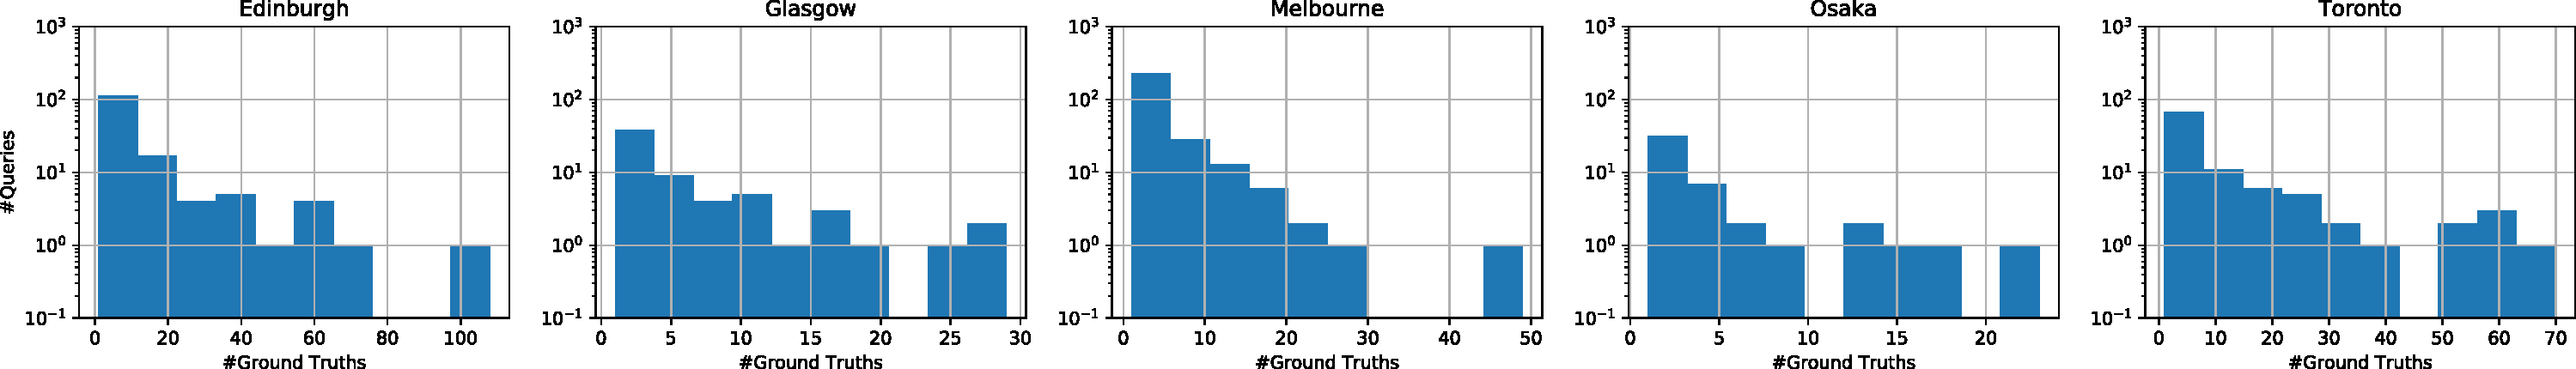
\includegraphics[width=\columnwidth]{hist.pdf}
	\caption{Histograms of the number of trajectories per query.}
	\label{fig:hist}
\end{figure}


\secmoveup
\subsection{Methods compared}
\textmoveup

We compare the performance of our methods to the following three baselines:
\begin{itemize}[leftmargin=0.125in]\itemmoveup
\parskip -.05em
	\item The \textsc{Random} baseline simply recommends a sequence of POIs by sampling uniformly at random from the whole set of POIs (without replacement).

	\item The stronger \textsc{Popularity} baseline recommends the top-$k$ most popular POIs i.e. the POIs that have been visited the most in the training set.

	\item \textsc{PoiRank}~\cite{cikm16paper} is a generalisation of \textsc{Popularity} which considers a number of POI features in addition to the popularity,
and trains a RankSVM model to learn a score for each POI. The top-$k$ scoring POIs are then used to construct a trajectory.
\end{itemize}\itemmoveup

To assess the viability of our structured prediction approach, and the necessity of our two extensions (normalising the loss per query and disallowing loops), we implemented the following versions of our structured prediction methods.
All variants predicts with the list Viterbi algorithm (Section~\ref{ssec:subtour}) to generate a path.
\begin{itemize}[leftmargin=0.125in]\itemmoveup
\parskip -.05em
	\item The structured prediction ({\sc SP}) method employs the vanilla structured SVM framework in order to learn a score for trajectories given a query.

	\item The structured recommendation ({\sc SR}) method extends the {\sc SP} method by additionally incorporating multiple ground truths into
	forming the constraints and adding them in cutting-plane algorithm,
	described in Section~\ref{ssec:sr} and \ref{ssec:SRinf}.
	%performing normalisation of the loss function per query,
	%so that we do not attempt to distinguish between multiple ground truths for the same query.

	\item The variants {\sc SPpath} and {\sc SRpath} extend the above methods by enforcing the constraint during training that sequences with loops are disallowed.
\end{itemize}\itemmoveup


\secmoveup
\subsection{Evaluation procedure}
\textmoveup

% leave-one-out evaluation (with query aggregation)
%As described in Section~\ref{sec:queryagg},
%To evaluate the performance of the various methods under comparison,
%we first group the trajectories  %according to queries that they conform to.
We then evaluate the performance of each algorithm using leave-one-query-out cross validation. That is, holding out each query $\x\pb{i}$, and also all of its relevant trajectories $\{\y\pb{ij}\}_{j=1}^{n^i}$ in each round.
where in each iteration of this procedure,
%one query and its associated trajectories serves as a test point, with all other trajectories for training.
%(Note that without this query aggregation, there will be considerable overlap between the train and test set, and simple nearest neighbour methods will be hard to outperform.)
% model selection (Monte Carlo CV) (with query aggregation): 90/10 random split for 5 times
Relevant hyper-parameters (e.g.\ the regularisation constant $C$) are tuned using Monte Carlo cross validation~\cite{burman1989comparative} on the training set.

We use three different measures to compare algorithm performances.
The {\bf F$_1$ score on points}~\cite{ijcai15} computes F$_1$ on the predicted versus seen points
without considering their relative order.
The {\bf F$_1$ score on pairs}~\cite{cikm16paper} is proposed to mitigate this by computing F$_1$ on all ordered pairs in the predicted versus groundtruth sequence. It is 1 iff both sequences agree completely.
The well-known rank correlation {\bf Kendall's $\tau$} (version $b$)~\cite{agresti2010analysis} computes the ratio of concordant (correctly ranked) pairs minus discordant pairs, over all ($\frac{1}{2}l(l-1)$) pairs.
\eat{
% evaluation metric: kendall's Tau (mention F1, pF1)
We use three performance measures to assess the test fold performance of each algorithm:
point-F$_1$ score~\cite{ijcai15},
pairs-F$_1$ score~\cite{cikm16paper},
and
Kendall's $\tau$ (version $b$)~\cite{kendall1945,agresti2010analysis}.
\TODO{explain point and pairs}

Kendall's $\tau$
essentially measures the fraction of pairs of POIs that are correctly ordered in the prediction and ground truth sequences,
with adjustment for ties.
In particular,
define the rank of POIs $\mathcal{P}$ in a trajectory $\mathbf{y} = (y_1,\dots,y_K)$ as
the position of the POI within the trajectory,
\begin{align*}
r_\mathbf{y} &= (r_1,\dots,r_j,\dots,r_{|\mathcal{P}|}), \\
r_j &= \sum_{k=1}^K (| \mathcal{P} | - k + 1)  \llb p_j = y_k \rrb, ~ j = 1, \dots, | \mathcal{P} |.
\end{align*}
The Kendall's $\tau$ score is then computed on $r_\mathbf{y}$ versus $r_\mathbf{\hat{y}}$.
Unlike the F$_1$ scores on points and pairs,
which only care about the set of correctly recommended POIs or POI pairs,
this metric taking both factors into account.
}

Structured recommendation problems aims to perform ranking on a very large $m^l$ labelset.
We adopt the practice of {\em best of top 10}~\cite{russakovsky2015imagenet} for reporting results. Or, predict top 10 trajectories and then report the best match of any in the top 10 to any trajectory in the ground truth set.
\eat{
As described previously, our methods are capable of recommending not merely a single trajectory,
but rather a list of trajectories.
While one can simply take the top recommended trajectory as the prediction,
this ignores the fact that there are likely multiple plausible trajectories for any given query.
Thus, for each performance measure $\mathrm{perf}$,
we take the maximum over all trajectories,
i.e.,
\begin{equation*}
%\tau_b^{(i)} =
\mathrm{perf}^{(i)}( \mathbf{y}, \hat{\mathbf{y}} ) =
\max_{(\mathbf{y}, \hat{\mathbf{y}}) \in \{\mathbf{y}^{(ij)}\}_{j=1}^{N_i} \times \{\hat{\mathbf{y}}^{(ij)}\}_{j=1}^k}
%\tau_b(r_\mathbf{y}, r_{\hat{\mathbf{y}}}),
\mathrm{perf}(\mathbf{y}, {\hat{\mathbf{y}}}),
\end{equation*}
where $\{\mathbf{y}^{(ij)}\}_{j=1}^{N_i}$ are the ground truths for query $\mathbf{x}^{(i)}$ and
$\{\hat{\mathbf{y}}^{(ij)}\}_{j=1}^k$ are the top-$k$ recommendations.
}

\secmoveup
\subsection{Results and discussion}
\label{sec:result}
\textmoveup

% !TEX root = ./main.tex

\begin{table*}[t]
\caption{Experimental results on trajectory recommendation datasets. The top three rows are baselines, and the bottom four are the methods proposed in this paper. Bolded entries correspond to the best performing method for each metric; italicised entries to the next best method. Higher scores are better.}
\label{tab:result}
\centering
%\setlength{\tabcolsep}{3pt} % tweak the space between columns
\small
\begin{tabular}{l|cc|cc|cc} \hline
                    & \multicolumn{2}{|c}{\textbf{Kendall's $\tau$}}
                    & \multicolumn{2}{|c}{\textbf{F$_1$ score on points}}
                    & \multicolumn{2}{|c}{\textbf{F$_1$ score on pairs}} \\ \cline{2-7}
                    & Osaka & Glasgow 
                    & Osaka & Glasgow  
                    & Osaka & Glasgow \\ \hline
\textsc{Random}     & $0.403\pm0.025$ & $0.410\pm0.032$  
                    & $0.430\pm0.021$ & $0.451\pm0.027$  
                    & $0.057\pm0.024$ & $0.136\pm0.037$ \\
\textsc{Popularity} & $0.567\pm0.034$ & $0.646\pm0.035$  
                    & $0.601\pm0.031$ & $0.681\pm0.032$  
                    & $0.277\pm0.051$ & $0.416\pm0.050$ \\
\textsc{PoiRank}    & $0.646\pm0.040$ & $0.736\pm0.030$  
                    & $0.678\pm0.037$ & $0.764\pm0.027$  
                    & $0.425\pm0.058$ & $0.550\pm0.047$ \\
\midrule
\textsc{SP}         & $0.796\pm0.037$ & $0.865\pm0.027$  
                    & $0.817\pm0.034$ & $0.878\pm0.024$  
                    & $0.665\pm0.055$ & $0.772\pm0.040$ \\
\textsc{SPpath}     & $0.794\pm0.035$ & $0.740\pm0.034$  
                    & $0.814\pm0.032$ & $0.764\pm0.030$  
                    & $0.653\pm0.054$ & $0.591\pm0.047$ \\
\textsc{SR}         & $\mathbf{0.814\pm0.034}$ & $\mathit{0.870\pm0.025}$  
                    & $\mathbf{0.832\pm0.031}$ & $\mathit{0.887\pm0.022}$ 
                    & $\mathit{0.673\pm0.053}$ & $\mathit{0.774\pm0.039}$ \\
\textsc{SRpath}     & $\mathit{0.805\pm0.036}$ & $\mathbf{0.877\pm0.025}$ 
                    & $\mathit{0.821\pm0.033}$ & $\mathbf{0.893\pm0.021}$ 
                    & $\mathbf{0.682\pm0.054}$ & $\mathbf{0.792\pm0.038}$ \\ \hline
\end{tabular}
\end{table*}


% experimental results
The performance of three baselines and four variants based on structured prediction on two datasets are shown in Table~\ref{tab:result}.
From these results, we can make the following key inferences that validate our contributions.

\textbf{Exploiting the structure of sequences helps}.
We find that all variants of our structured prediction methods achieve better performance than existing baselines.
This indicates that the basis of our approach -- reducing sequence recommendation to a structured prediction problem -- is sensible, and has empirical benefit.

\textbf{Accounting for multiple ground truths helps}.
We find that \textsc{SR} always performs better than \textsc{SP},
and similarly for the {\sc path} variants of both methods.
This indicates that our first extension -- explicitly modelling multiple ground truths helps recommendation -- is important to achieve good performance.
(We note that even without this correction, our structured methods outperform baselines.)

\textbf{Eliminating loops during training helps}.
We find that {\sc SRpath} improves performance further of the {\sc SR} method,
as indicated by the F$_1$ score on pairs.
This indicates that our second extension -- explicitly performing sub-tour elimination in training -- is important to further improve performance.
Interestingly,
this advantage does \emph{not} take effect if the multiple ground truths are not modelled explicitly,
with the performance of the {\sc SP} method largely unaffected.

\textbf{An illustrative example}. Figure~\ref{fig:example} consist of an example that illustrates the difference among the different algorithm variants. The query requires the trajectory to start from the middle point and be of length 2.
\textsc{PoiRank} regards points at the lower right and upper left be of the highest rank, but did not consider their compatibility (\ie pairwise features). {\sc SP} and {\sc SR} hits one edge out of the two the groundtruth (green edge), while {\sc SRpath} hits both edges for two valid trajectories after taking all factors into account.

Overall, these results indicate that our structured prediction approach to the problem has
benefits over non-structured approaches,
and that our extensions to the vanilla structured approach are important to further improve performance.

%\subsection{Example}
%\label{sec:example}

\begin{figure*}[t]
	\centering
	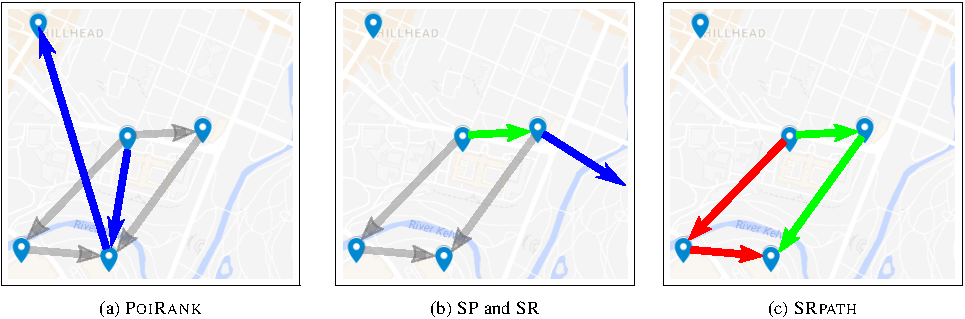
\includegraphics[width=0.9\textwidth]{example.pdf}
	\caption{Example of structured recommender versus baseline on a query with two ground truths as shown in Figure (c).
             (a) \textsc{PoiRank} cannot make a recommendation related to any of the ground truths;
             (b) \textsc{SP} and \textsc{SR} recommend a better trajectory than \textsc{PoiRank}, but not fully consistent with the ground truths;
             (c) \textsc{SRpath} hit both ground truths at rank 3 and 5 respectively.}
	\label{fig:example}
\end{figure*}


% !TEX root=./main.tex

\section{Related work}
\label{sec:related}

We contrast the problem setting and approach of this paper to a number of sub-fields in the recommender systems and machine learning literature.

%
\subsection{Recommender systems}

There is a rich body of work on recommender systems,
with the 
Netflix prize~\citep{Netflix} encapsulating the canonical problem that concerns most research in this field:
the recommendation of \emph{static} content such as books or movies from some large database~\citep{Goldberg:1992,Resnick:1994,Konstan:1997,Sarwar:2001,Koren:2010}.
Matrix factorisation methods have proven particularly effective for such problems~\citep{Koren:2009}.
The latter are a prototypical example of a \emph{collaborative filtering} approach to recommendation,
wherein one exploits the ``wisdom of the crowd'' implicit in the preferences of several users.

Standard matrix factorisation methods
have been extended to tackle
diverse problem settings such as
time-varying preferences~\citep{Koren:2009b} and implicitly provided feedback~\citep{Hu:2008,Rendle:2009}.
However,
the setting of recommending \emph{structured content},
such as trajectories as considered in this paper,
has received less attention but for a few exceptions (see below).
There are clear challenges with applying matrix factorisation techniques in our problem.
First, most users are only associated with a single trajectory, which defeats any hope of inferring a complex preference embedding for them.
Second, even if one had access to multiple trajectories per user, it is unclear how to find a latent embedding for entire trajectories,
as there are exponentially many possible values for the latter.


%
\subsection{Structured content recommendation}

The recommendation of structured content has
been studied in three distinct subfields.
The first is work on recommending the next item a user might like to purchase, given the sequence of their shopping basket purchases~\citep{Rendle:2010,Wang:2015}.
The canonical approach here is to apply the matrix factorisation idea to the Markov chain of transitions between items.
The success of this method relies on the fact that one is only interested in predicting sequences one element at a time, so that latent embeddings for each item may be found.

The second is work on recommending song playlists to users, given a query song~\citep{McFee:2011,chen2012playlist}.
The canonical approach here is to 
learn a latent representation of songs from historical playlist data,
and exploit a Markovian assumption on the song transitions.
While a reasonable first order approximation, this assumption limits the modelling power of such approaches.

The third is prior work on travel route recommendation, which we survey in detail.


%
\subsection{Travel route recommendation}

Recommendation problems involving travel routes have received considerable interest of late~\cite{bao2015recommendations,zheng2015trajectory,zheng2014urban}.
There are, roughly, three problem settings that have been studied.
The first setting is \emph{point of interest} (\emph{POI}) \emph{recommendation}.
Here, one simply wishes to rank various POIs in a city in order of how ``interesting'' they are to a given visitor,
exploiting
available metadata for each POI.
Typically, this problem is tackled via 
collaborative filtering on user-location affinity~\cite{shi2011personalized,lian2014geomf,liu2014exploiting,yuan2013timeaware,hsieh2014mining,gao2013temporal,yuan2014graph}.

The second setting is \emph{next location recommendation}.
Here, given the sequence of a traveller's partial tour through a city,
the goal is to recommend which POI the traveller should visit next.
This can be understood as a variant of POI recommendation with strong contextual information provided.
Typically, this problem is tackled via 
incorporating Markov chains into collaborative filtering~\cite{fpmc10,ijcai13,zhang2015location},
%quantifying tourist traffic flow between points-of-interest~\cite{zheng2012patterns},
%formulating a binary decision or ranking problem~\cite{baraglia2013learnext}, and predicting the next location with
or sequence models such as recurrent neural networks~\cite{aaai16}.

The third setting is trajectory recommendation,
which is our focus in this paper.
Typically, this problem is tackled via 
a heuristic combination of locations and routes~\cite{lu2010photo2trip,ijcai15,lu2012personalized}, or
by solving an optimisation problem that does not exploit historical data~\cite{gioniswsdm14,chen2015tripplanner}.


%
\subsection{Learning to rank}

% AKM: probably can omit this stuff as I dunno how to frame it properly

The trajectory recommendation problem can be related at an abstract level to the label ranking problem~\citep{Dekel:2003},
where the input comprises a query and a corresponding graph as a label.
The goal in such problems is to learn a ranking over the nodes of the graph,
which is similar to our setting;
however, these are typically not learned using structured prediction models.

Our problem can also be related to the listwise ranking approach in information retrieval~\citep{Cao:2007},
which attempts to learn a good set of results for a query by exploiting structure embedded in the entire set of results.
One contribution of this work is in casting trajectory recommendation as such a structured prediction problem, as opposed to
pointwise and pairwise approaches considered in previous work.

% !TEX root = ./main.tex

\section{Conclusion}

We showed how the problem of sequential recommendation,
which arises in contexts such as
recommending a playlist of songs, or a trajectory of points-of-interest in a city,
can be viewed as a structured prediction problem.
We proposed a structured support vector machine for this recommendation task, with two important changes:
first, we modified the training objective to account for the existence of multiple ground truths;
second, we modified the prediction and loss augmented inference procedures to avoid predicting loops in the sequence via an extension of the classic Viterbi algorithm.
Experiments on two real-world trajectory recommendation datasets showed the benefits of our approach over existing, non-structured recommendation approaches.

There are several important directions for future work.
First, it is of interest to assess the viability of probabilistic approaches to structured prediction,
such as the conditional random field and maximum entropy Markov model.
Second, extending our approaches to additionally capture latent user- and POI-representations, when sufficient personalised data of this type is available, would be of interest.
Third, applying structured prediction approaches to other sequential prediction problems, such as playlist generation, may indicate similar benefits as observed in the trajectory recommendation problem.
%Third, it will be beneficial to consider loss-augmented inference for more complex performance measures.


% Acknowledgements should only appear in the accepted version.
%\section*{Acknowledgements}
%
%\textbf{Do not} include acknowledgements in the initial version of
%the paper submitted for blind review.

\bibliographystyle{icml2017}
\bibliography{ref,ref_aditya}

\clearpage
\onecolumn

\appendix
\section{Supplementary material to Sequence Recommendation with Structured Prediction}
\label{sec:supplement}

\subsection{List Viterbi}
\label{sec:listviterbi-supp}

We require a top-$k$ decoding of a sequence for three situations:
\begin{enumerate}
  \item To perform top-$k$ inference during the prediction phase
  \item To perform loss-augmented inference that includes avoiding all $n_i$ ground truth
    trajectories corresponding to the $i$th example.
  \item To find a decoding that does not have loops, that is to find a path
    and not a walk (with subtours).
\end{enumerate}

There are two general approaches for generalising Viterbi decoding to when we require $k$
sequences to be decoded: by maintaining $k$ paths through the trellis while decoding; or by
careful book keeping of the best $k-1$ paths through the trellis found so far and avoiding them.
We choose the latter approach as it is more memory efficient.

The list Viterbi approach~\cite{nilsson2001sequentially,seshadri1994list} maintains
a heap of potential solutions, which are then checked for the desired property (for example
whether there are subtours). Once the requisite number of trajectories with the desired
property are found, the algorithm terminates (for example once one trajectory without subtours
is found). The heap is initialised by running forward-backward
(Algorithm~\ref{alg:forward-backward})
followed by Viterbi (Algorithm~\ref{alg:viterbi}).

\begin{algorithm}[htbp]
\caption{Forward-backward procedure~\cite{rabiner1989tutorial}}
\label{alg:forward-backward}
\begin{algorithmic}[1]
  \STATE $\forall p_j \in \mathcal{P},~ \alpha_t(p_j) =
          \begin{cases}
          0,~ t = 1 \\
          \max_{p_i \in \mathcal{P}} \left\{ \alpha_{t-1}(p_i) + \mathbf{w}_{ij}^\top \Psi_{ij}(\mathbf{x}, p_i, p_j) +
          \mathbf{w}_j^\top \Psi_j(\mathbf{x}, p_j) \right\},~ t=2,\dots,K
          \end{cases}$

  \STATE $\forall p_i \in \mathcal{P},~ \beta_t(p_i) =
          \begin{cases}
          0,~ t = K \\
          \max_{p_j \in \mathcal{P}} \left\{ \mathbf{w}_{ij}^\top \Psi_{ij}(\mathbf{x}, p_i, p_j) +
          \mathbf{w}_j^\top \Psi_j(\mathbf{x}, p_j) + \beta_{t+1}(p_j) \right\},~ t = K-1,\dots,1
          \end{cases}$

  %\STATE $\forall p_i \in \mathcal{P},~ f_t(p_i) = \alpha_t(p_i) + \beta_t(p_i),~ t = 1,\dots,K$
  \STATE $\forall p_i, p_j \in \mathcal{P},~ f_{t,t+1}(p_i, p_j) = \alpha_t(p_i) + \mathbf{w}_{ij}^\top \Psi_{ij}(\mathbf{x}, p_i, p_j) +
                                \mathbf{w}_j^\top \Psi_j(\mathbf{x}, p_j) + \beta_{t+1}(p_j),~ t = 1,\dots,K-1$
\end{algorithmic}
\end{algorithm}

\begin{algorithm}[htbp]
\caption{Viterbi}
\label{alg:viterbi}
\begin{algorithmic}[1]
  \STATE $y_t^1 = \begin{cases}
                  s,~ t = 1 \\
  %                \argmax_{p \in \mathcal{P}} \left\{ f_{1,2}(s, p) \right\},~ t = 2, \\
                  \argmax_{p \in \mathcal{P}} \left\{ f_{t-1,t}(y_{t-1}^1, p) \right\},~ t = 2,\dots,K
                  \end{cases}$

  %\STATE $r^1 = \max_{p \in \mathcal{P}} \left\{ f_K(p) \right\}~~~ \triangleright$ $r^1$ is the score/priority of $\mathbf{y}^1$
  \STATE $r^1 = \max_{p \in \mathcal{P}} \left\{ \alpha_{K}(p) \right\}~~~ \triangleright$ $r^1$ is the score/priority of $\mathbf{y}^1$
\end{algorithmic}
\end{algorithm}

Given an existing heap containing potential trajectories,
list Viterbi maintains a set of POIs to exclude $S$, which is updated
sequentially by considering the front sequence of the heap.

Recall that for trajectory recommendation we are given the query $\mathbf{x}=(s, K)$, where
$s$ is the starting POI from the set of POIs $\mathcal{P}$,
and $K$ is the desired length of the trajectory.
We assume the score function is of the form $\mathbf{w}^\top \Psi$ where $\Psi$ is the joint
feature vector. $\mathbf{w}$ could be the value of the weight in the current iteration in training,
or the learned weight vector during prediction.

\begin{algorithm}[htbp]
\caption{The list Viterbi algorithm for inference~\cite{nilsson2001sequentially,seshadri1994list}}
\label{alg:listviterbi}
\begin{algorithmic}[1]
\STATE \textbf{Input}: $\mathbf{x}=(s, K),~ \mathcal{P},~ \mathbf{w},~ \Psi$
%\STATE Initialise score matrices $\alpha,~ \beta,~ f_t,~ f_{t, t+1}$, a max-heap $H,~ k=0$.
\STATE Initialise score matrices $\alpha,~ \beta,~ f_{t, t+1}$, a max-heap $H$, result set $R$, $k=0$.
\STATE $\triangleright$ Do the forward-backward procedure~\cite{rabiner1989tutorial}
\STATE $\triangleright$ Identify the best (scored) trajectory $\mathbf{y}^1=(y_1^1,\dots,y_K^1)$
  with Viterbi. This may be a trajectory that violates the desired condition.
\STATE $H.\textit{push}\left(r^1,~ (\mathbf{y}^1, \textsc{nil}, \emptyset) \right)$
\STATE Set $R=\emptyset$, the list of trajectories to be returned.
\WHILE{$H \ne \emptyset$ \textbf{and} $k < \,|\mathcal{P}|^{K-1} - \prod_{t=2}^K (|\mathcal{P}|-t+1)$}
    \STATE $r^k,~ (\mathbf{y}^k, I, S) = H.\textit{pop}()~~~ \triangleright$
           $r^k$ is the score of $\mathbf{y}^k=(y_1^k,\dots,y_K^k)$, $I$ is the partition index, and $S$ is the exclude set
    \STATE $k = k + 1$
    \STATE Add $\mathbf{y}^k$ to $R$ if it satisfies the desired property
    \RETURN $R$ if it contains the required number of trajectories
    \STATE $\bar{I} = \begin{cases}
                      2,~ I = \textsc{nil} \\
                      I,~ \text{otherwise}
                      \end{cases}$

    \FOR{$t = \bar{I},\dots,K$}
        \STATE $\bar{S} = \begin{cases}
                          S \cup \{ y_t^k \},& t = \bar{I} \\
                          \{ y_t^k \},& \text{otherwise}
                          \end{cases}$

        \STATE $\bar{y}_j = \begin{cases}
                            y_j^k,& j=1,\dots,t-1 \\
                            %\argmax_{p \in \mathcal{P} \setminus \textit{new\_exclude\_set}} f_{t-1,t}(y_{t-1}^k, p),~ j=t \\
                            \argmax_{p \in \mathcal{P} \setminus \bar{S}} \left\{ f_{t-1,t}(y_{t-1}^k, p) \right\},& j=t \\
                            \argmax_{p \in \mathcal{P}} \left\{ f_{j-1, j}(\bar{y}_{j-1}, p) \right\},& j=t+1,\dots,K
                \end{cases}$
        \STATE $\bar{r} = \begin{cases}
                          f_{t-1,t}(y_{t-1}^k, \bar{y}_t),&I = \textsc{nil} \\
                          r^k + f_{t-1,t}(y_{t-1}^k, \bar{y}_t) - f_{t-1,t}(y_{t-1}^k, y_t^k), &\text{otherwise}
                          \end{cases}$

        $H.\textit{push}\left(\bar{r}, (\bar{\mathbf{y}}, t, \bar{S}) \right)$
    \ENDFOR
\ENDWHILE
\end{algorithmic}
\end{algorithm}

\clearpage
\subsection{Photo Trajectory Dataset}
\label{sec:feature}

In the interests of reproducibility we present further details of our empirical experiment.

The POI and query specific features extracted from trajectories are shown in Table~\ref{tab:poifeature},
features that describe the transition preference between different POIs are shown in Table~\ref{tab:tranfeature}.

\begin{table*}[ht]
\caption{Features of POI $p$ with respect to query $(s,K)$}
\label{tab:poifeature}
\centering


\setlength{\tabcolsep}{10pt} % tweak the space between columns
\begin{tabular}{l|l} \hline
\textbf{Feature}       & \textbf{Description} \\ \hline
\texttt{category}      & one-hot encoding of the category of $p$ \\
\texttt{neighbourhood} & one-hot encoding of the POI cluster that $p$ resides in \\
\texttt{popularity}    & logarithm of POI popularity of $p$ \\
\texttt{nVisit}        & logarithm of the total number of visit by all users at $p$ \\
\texttt{avgDuration}  & logarithm of the average visit duration at $p$ \\
\hline
%\texttt{nOccurrence}            & the number of times $p$ occurred in a trajectory that satisfies the query \\ DON'T know given new query

\texttt{trajLen}           & trajectory length $K$, i.e., the number of POIs required \\
\texttt{sameCatStart}      & $1$ if the category of $p$ is the same as that of $s$, $-1$ otherwise \\
\texttt{sameNeighbourhoodStart} & $1$ if $p$ resides in the same POI cluster as $s$, $-1$ otherwise \\
\texttt{diffPopStart}    & real-valued difference in POI popularity of $p$ from that of $s$ \\
\texttt{diffNVisitStart}        & real-valued difference in the total number of visit at $p$ from that at $s$ \\
\texttt{diffDurationStart}  & real-valued difference in average duration at $p$ from that at $s$ \\
\texttt{distStart}          & distance between $p$ and $s$, calculated using the Haversine formula \\
\hline
\end{tabular}
\end{table*}



\begin{table}[ht]
\caption{POI features used to estimate the (feature-wise) transition probabilities}
\label{tab:tranfeature}
\centering
\setlength{\tabcolsep}{2pt} % tweak the space between columns
\begin{tabular}{l|l} \hline
\textbf{Feature}       & \textbf{Description} \\ \hline
\texttt{category}      & category of POI \\
\texttt{neighbourhood} & the cluster that a POI resides in \\
\texttt{popularity}    & (discretised) popularity of POI \\
\texttt{nVisit}        & (discretised) total number of visit at POI \\
\texttt{avgDuration}  & (discretised) average duration at POI \\ \hline
\end{tabular}
\end{table}


\clearpage
\subsection{Evaluation procedures}
\label{sec:metric}

To evaluate the performance of a certain recommendation algorithm,
we need to measure the similarity (or loss) given prediction $\hat{\mathbf{y}}$
and ground truth $\mathbf{y}$.

\begin{itemize}
  \item F$_1$ score on points~\cite{ijcai15}, where we care about the set of correctly recommended POIs.
      Let $\texttt{set}(\mathbf{y})$ denote the set of POIs in trajectory $\mathbf{y}$, F$_1$ score on points is defined as
\begin{equation*}
F_1(\mathbf{y}, \hat{\mathbf{y}}) = \frac{2  P_{\textsc{point}}  R_{\textsc{point}}}{P_{\textsc{point}} + R_{\textsc{point}}}
%~~\text{where}~
%P_{\textsc{point}} = \frac{| \texttt{set}(\hat{\mathbf{y}}) \cap \texttt{set}(\mathbf{y}) |}{| \texttt{set}(\hat{\mathbf{y}}) |}~\text{and}~
%R_{\textsc{point}} = \frac{| \texttt{set}(\hat{\mathbf{y}}) \cap \texttt{set}(\mathbf{y}) |}{| \texttt{set}(\mathbf{y}) |}.
\end{equation*}
If $| \hat{\mathbf{y}} | = | \mathbf{y} |$, this metric is just the unordered Hamming loss,
i.e., Hamming loss between two binary indicator vectors of size $| \mathcal{P} |$.

\item F$_1$ score on pairs~\cite{cikm16paper}, where we care about the set of correctly predicted POI pairs,
\begin{equation*}
\text{pairs-F}_1(\mathbf{y}, \hat{\mathbf{y}}) = \frac{2 P_{\textsc{pair}} R_{\textsc{pair}}}{P_{\textsc{pair}} + R_{\textsc{pair}}}
%~~\text{where}~
%P_{\textsc{pair}} = \frac{N_c} {| \texttt{set}(\hat{\mathbf{y}}) | (| \texttt{set}(\hat{\mathbf{y}}) | - 1) / 2}~\text{and}~
%R_{\textsc{pair}} = \frac{N_c} {| \texttt{set}(\mathbf{y}) | (| \texttt{set}(\mathbf{y}) | - 1) / 2},
\end{equation*}
and $N_c = \sum_{j=1}^{| \mathbf{y} | - 1} \sum_{k=j+1}^{| \mathbf{y} |} \llb y_j \prec_{\bar{\mathbf{y}}} y_k \rrb$,
here $y_j \prec_{\bar{\mathbf{y}}} y_k$ denotes that POI $y_j$ appears before POI $y_k$ in trajectory $\bar{\mathbf{y}}$.
We define pairs-F$_1 = 0$ when $N_c = 0$.

\end{itemize}

However, if we cast a trajectory $\mathbf{y} = (y_1,\dots,y_K)$ as a ranking of POIs in $\mathcal{P}$,
where $y_k$ has a rank $| \mathcal{P} | - k + 1$ and any other POI $p \notin \mathbf{y}$ has a rank $0$ ($0$ is an arbitrary choice).
We can make use of ranking evaluation metrics such as Kendall's $\tau$ by taking care of ties in ranks.

\subsection{Kendall's $\tau$ with ties}

Given a prediction $\hat{\mathbf{y}} = (\hat{y}_1, \hat{y}_2, \dots, \hat{y}_K)$ and ground truth $\mathbf{y} = (y_1, y_2, \dots, y_K)$,
for a specific ordering of POIs $(p_1, p_2, \dots, p_{|\mathcal{P}|})$,
we produce two ranks according to $\mathbf{y}$ and $\hat{\mathbf{y}}$,
\begin{align*}
r_i       &= \sum_{j=1}^K (| \mathcal{P} | - j + 1)  \llb p_i = y_j \rrb,~
i = 1, \dots, | \mathcal{P} | \\
\hat{r}_i &= \sum_{j=1}^K (| \mathcal{P} | - j + 1)  \llb p_i = \hat{y}_j \rrb,~
i = 1, \dots, | \mathcal{P} |
\end{align*}
where POIs not in $\mathbf{y}$ will have a rank of $0$ in $r$ and similarly in $\hat{r}$.
Then we have
\begin{align*}
C &= \frac{1}{2} \sum_{i,j} \left(\llb r_i < r_j \rrb  \llb \hat{r}_i < \hat{r}_j \rrb +
     \llb r_i > r_j \rrb  \llb \hat{r}_i > \hat{r}_j \rrb \right), \\
D &= \frac{1}{2} \sum_{i,j} \left(\llb r_i < r_j \rrb  \llb \hat{r}_i > \hat{r}_j \rrb +
     \llb r_i > r_j \rrb  \llb \hat{r}_i < \hat{r}_j \rrb \right), \\
T_{\mathbf{y}} &= \frac{1}{2} \sum_{i \ne j} \llb r_i = r_j \rrb \\
               &= \frac{1}{2} \sum_{i \ne j} \llb r_i = 0 \rrb  \llb r_j = 0 \rrb \\
               &= \frac{1}{2} \left( |\mathcal{P}| - K \right) \left( |\mathcal{P}| - K - 1 \right), \\
T_{\hat{\mathbf{y}}} &= \frac{1}{2} \sum_{i \ne j} \llb \hat{r}_i = \hat{r}_j \rrb \\
                     &= \frac{1}{2} \sum_{i \ne j} \llb \hat{r}_i = 0 \rrb  \llb \hat{r}_j = 0 \rrb \\
                     &= \frac{1}{2} \left( |\mathcal{P}| - K \right) \left( |\mathcal{P}| - K - 1 \right), \\
T_{\mathbf{y},\hat{\mathbf{y}}} &= \frac{1}{2} \sum_{i \ne j} \llb r_i = r_j \rrb  \llb \hat{r}_i = \hat{r}_j \rrb \\
                                &= \frac{1}{2} \sum_{i \ne j} \llb r_i = 0 \rrb  \llb r_j = 0 \rrb
                                   \llb \hat{r}_i = 0 \rrb  \llb \hat{r}_j = 0 \rrb.
\end{align*}
Kendall's $\tau$ (version $b$)~\cite{kendall1945,agresti2010analysis} is
\begin{equation*}
\tau_b(\mathbf{y}, \hat{\mathbf{y}}) = \frac{C - D}{\sqrt{(C + D + T) (C + D + U)}},
\end{equation*}
where $T = T_{\mathbf{y}} - T_{\mathbf{y},\hat{\mathbf{y}}}$ and $U = T_{\hat{\mathbf{y}}} - T_{\mathbf{y},\hat{\mathbf{y}}}$.

Furthermore, F$_1$ score on points can be written as
\begin{equation*}
F_1(\mathbf{y}, \hat{\mathbf{y}}) = \frac{1}{K} \sum_i \llb r_i > 0 \rrb  \llb \hat{r}_i > 0 \rrb,
\end{equation*}
and F$_1$ score on pairs can be written as
\begin{align*}
& \text{pairs-F}_1(\mathbf{y}, \hat{\mathbf{y}}) \\
&= \left( \frac{1}{2} \sum_{i,j} \llb r_i < r_j \rrb  \llb r_i > 0 \rrb \llb \hat{r}_i < \hat{r}_j \rrb  \llb \hat{r}_i > 0 \rrb \right. \\
&  \left. ~+ \frac{1}{2} \sum_{i,j} \llb r_i > r_j \rrb  \llb r_j > 0 \rrb \llb \hat{r}_i > \hat{r}_j \rrb  \llb \hat{r}_j > 0 \rrb \right)
   \cdot \frac{1}{K(K-1)/2} \\
&= \frac{\sum_{i,j} \llb r_i < r_j \rrb  \llb r_i > 0 \rrb \llb \hat{r}_i < \hat{r}_j \rrb  \llb \hat{r}_i > 0 \rrb +
         \sum_{i,j} \llb r_i > r_j \rrb  \llb r_j > 0 \rrb \llb \hat{r}_i > \hat{r}_j \rrb  \llb \hat{r}_j > 0 \rrb}
        {K(K-1)}
\end{align*}


\end{document}
